%!TEX root = paper.tex

\subsection{Packages}

%\subsubsection{Package Files}
\begin{figure}
	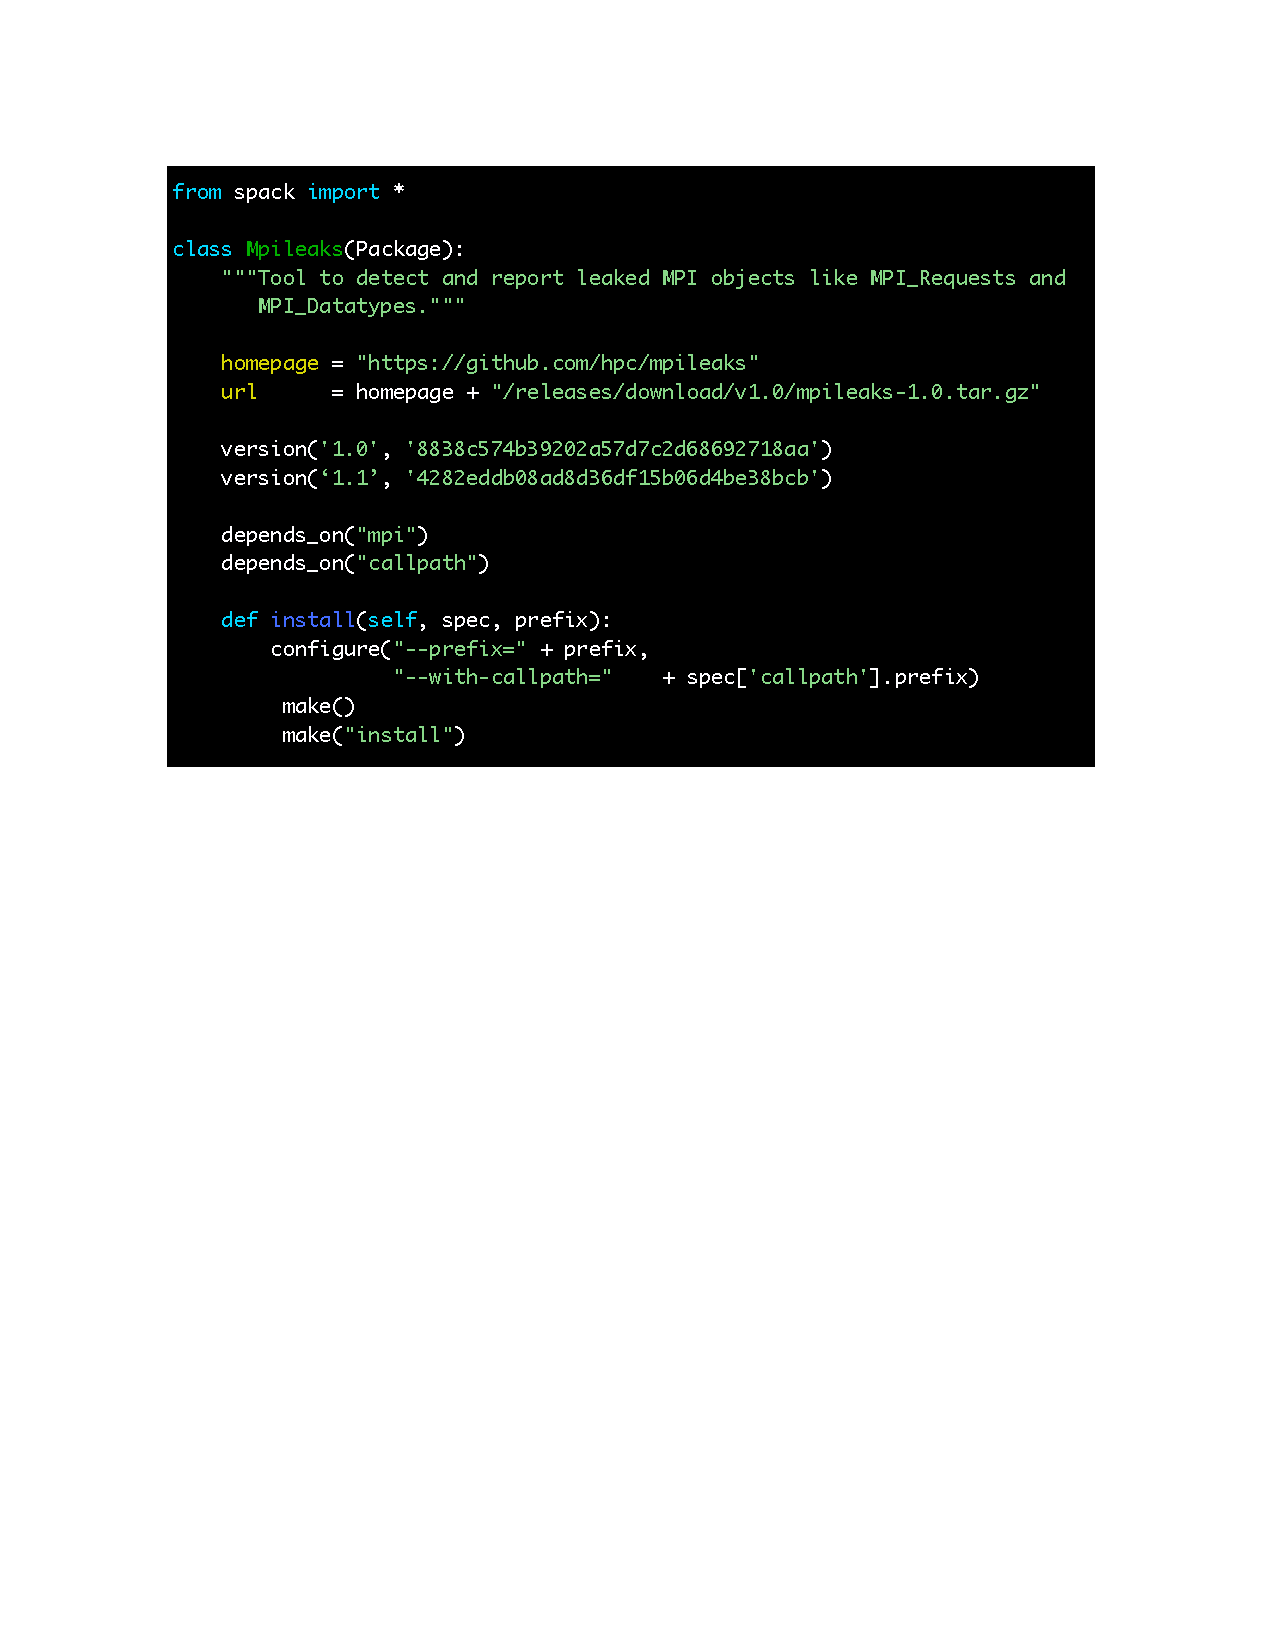
\includegraphics[width=\columnwidth]{code/mpileaks.pdf}
	\caption{
		Spack package for the {\tt mpileaks} tool.
		\label{fig:mpileaks}
	}
\end{figure}

Spack comprises many packages, and each describes how to build a software
artifact.  Each package is a class written in pure Python, but Spack uses
a simple, embedded domain-specific language (DSL) to make packaging easier.
Spack's DSL adds directives such as {\tt depends\_on}, {\tt version},
{\tt provides}, and {\tt extends}, in order to add metadata to package classes.

Figure~\ref{fig:mpileaks} shows the package for the \mpileaks tool.
Inside the {\tt MpiLeaks} class, the package provides a text description
and a homepage, as well as 
a download URL.  Next, two {\tt version} directives identify known versions
of the package, and checksums so that they can be downloaded safely.
Below this, three {\tt depends\_on}
directives indicate prerequisites that must be installed before \mpileaks.
Last, each package defines an {\tt install()} method, which contains the
commands used to build the package.

Most package managers fix a single version in a package file, but Spack packages
are {\it parameterized} by version.  In the figure, we see that the {\tt mpileaks}
package specifies two versions.  A user can safely install either by 
specifying it on the command line.  In our experience, however, users
frequently want bleeding-edge versions, and package managers frequently lag 
behind the latest releases.  Spack therefore has a capability to extrapolate
the latest URL, using the {\tt url} attribute as a model\footnote{This works
for consistently named URLs, and it can be specified per-version for packages
with inconsistent naming.}.
The user can ask for an unknown version on the command line and still
successfully download and install it.  Spack can also use the same model to
scrape webpages and find new versions. 

\subsubsection{Installation Environment}

%{\bf Reproducibility.}
%\paragraph{Reproducibility}
Spack is intended to build a consistent HPC stack for our multi-user
environment, and reproducible builds are one of our design goals.
Experience at LLNL has shown that it is vexingly difficult to reproduce
a build manually.
%
Many packages used at LLNL have a profusion of build options, and specifying them 
correctly often requires tedious experimentation.  This is due to lack of
build standards and to the diversity of HPC environments.  
For example, in some packages that depend on the {\tt Silo} library,
the {\tt ---with-silo} parameter takes a path to {\tt Silo}'s prefix.
In others, it takes the {\tt include} and {\tt lib} subdirectories,
separated by a comma.
The {\tt install()} method in Spack's package files allows us to record
precise build incantations for later reuse.

%{\bf Environment isolation.}
\paragraph{Environment isolation}
In addition to command line issues, we
frequently encounter errors due to inconsistencies between the environment of
the package installer and the package user.
%
For example, there are two versions of the {\tt libelf} library used by
LLNL performance tools. One is distributed with RedHat Linux, but another
publicly available version has the same API but an incompatible ABI.
Failure to specify the right version at build time has caused many
inexplicable crashes.
%
Spack manages the build environment by running {\tt install} invocation
in a new process.  It helps packages find dependencies 
correctly, by setting
{\tt PATH}, {\tt PKG\_CONFIG\_PATH}, {\tt CMAKE\_PREFIX\_PATH}, and
{\tt LD\_LIBRARY\_PATH} to include the dependencies of the current build.
These variables are commonly used by build systems to locate dependencies,
and setting them helps to ensure that incorrect libraries are not detected.
The isolated build environment also gives package authors 
free reign to set build-specific environment variables without interfering
with other packages.


%{\bf Compiler wrappers and RPATHs.}
\paragraph{Compiler wrappers and RPATHs}
Finding compilers at build time is not the only obstacle to reproducible
behavior.  As mentioned in Section~\ref{sec:motivation}, it is also important
for binaries to be able to find dependency libraries at {\it runtime}.
One of the most frequent user errors at LC is improper library configuration.
Users frequently do not know what libraries a package was built with, and 
it is difficult for them to construct a suitable {\tt LD\_LIBRARY\_PATH} for
a package that was built by someone else.  Because of frequent support calls,
we typically add {\tt RPATHs} to public software installations, so that paths
to dependencies are embedded in binaries and so that users do not have to know
this information to run installed software correctly.

Spack manages {\tt RPATH} settings and other build policies with
{\it compiler wrappers}. 
In each isolated {\tt install} environment, Spack sets the standard 
environment variables
{\tt CC}, {\tt CXX}, {\tt F77}, and {\tt FC} to point to its own compiler
wrapper scripts.  These variables are used by most build systems to select
C, C++, and Fortran compilers, so they are generally picked up 
automatically\footnote{If builds do not respect {\tt CC}, {\tt CXX}, etc.,
wrappers can typically be added as arguments or inserted into Makefiles
by {\tt install}.}.
When run, the wrappers insert include ({\tt -I}), library ({\tt -L}), and 
{\tt RPATH} ({\tt -Wl,-rpath} or similar) flags into the argument list.
These point to the {\tt include} and {\tt lib} directories of dependency
library installations, where needed headers and libraries are typically located.
After the modified argument list is constructed, the wrappers delegate it
to the real compiler to execute.

Spack's compiler wrappers have a number of useful effects.  First, they allow
Spack to transparently parameterize the compiler for most builds. 
Spack users to easily request a build with a new compiler swapped in.
Second, they enforce the use of {\tt RPATHs} in
installed binaries.  This causes applications built by Spack to run correctly
{\it regardless of the environment}.  Third, because compiler wrappers add 
header and library search paths for dependencies, header and library detection
tests run by most build systems succeed automatically, {\it without}
the need to use special arguments for nonstandard locations.  {\tt configure}
commands in Spack's {\tt install} function can have fewer arguments, and can
be written as they would be for system installs.  This reduces complexity
for package maintainers and enforces consistent, reproducible
build policies across packages.  Finally, because Spack has control over the 
wrappers, package authors can programmatically filter the compiler flags
used by software build systems, a useful last resort when porting to
bleeding-edge platforms or new, esoteric compilers.

\subsubsection{Environment Module Integration}
	\todo{.5 page}









\begin{verbatim}
module disadvantages:
	- lmod solves a lot of problems
	- not on all systems
		- users often run from just a path.
		- not guaranteed that LD_LIBRARY_PATH, etc will
		  be set correctly.

- Lmod assumes build & submit environment must match
	- users often have NO IDEA what environment a package
	  was built with
	- multiple apps may be built with different stacks
	- combining them in a workflow is difficult with modules
		(need to know right incantation)

	- TACC implements a rather complicated mapping back to
	    the build env (Lmod CheckExec)
	

- Spack solves the matrix problem mentioned in the Lmod
    presentation (slide 98)
	- hierarchy is nasty -- every branch represents a
	  greedy choice
	- might NEED a specific version of ONE dependency
	  that is not supported in the tree
	  => SPACK!

- libmesh
	- boost, petsc, trilinos, grvy, etc.
\end{verbatim}










